\documentclass{article}
\usepackage[utf8]{inputenc}

\usepackage{float}
\usepackage{natbib}
\usepackage{graphicx}
\usepackage[export]{adjustbox}
\usepackage{multirow}
\usepackage{hyperref}
\usepackage{titlesec}
\usepackage{ragged2e}


\documentclass{article}
\usepackage{bera}% optional: just to have a nice mono-spaced font
\usepackage{listings}
\usepackage{xcolor}

\colorlet{punct}{red!60!black}
\definecolor{background}{HTML}{EEEEEE}
\definecolor{delim}{RGB}{20,105,176}
\colorlet{numb}{magenta!60!black}

\lstdefinelanguage{json}{
    basicstyle=\normalfont\ttfamily,
    numbers=left,
    numberstyle=\scriptsize,
    stepnumber=1,
    numbersep=8pt,
    showstringspaces=false,
    breaklines=true,
    frame=lines,
    backgroundcolor=\color{background},
    literate=
     *{0}{{{\color{numb}0}}}{1}
      {1}{{{\color{numb}1}}}{1}
      {2}{{{\color{numb}2}}}{1}
      {3}{{{\color{numb}3}}}{1}
      {4}{{{\color{numb}4}}}{1}
      {5}{{{\color{numb}5}}}{1}
      {6}{{{\color{numb}6}}}{1}
      {7}{{{\color{numb}7}}}{1}
      {8}{{{\color{numb}8}}}{1}
      {9}{{{\color{numb}9}}}{1}
      {:}{{{\color{punct}{:}}}}{1}
      {,}{{{\color{punct}{,}}}}{1}
      {\{}{{{\color{delim}{\{}}}}{1}
      {\}}{{{\color{delim}{\}}}}}{1}
      {[}{{{\color{delim}{[}}}}{1}
      {]}{{{\color{delim}{]}}}}{1},
}




\begin{document}
\title{COS301 Team Gamma: Android Frontend (Integration Team)}
\begin{figure}
    \centering
    
\includegraphics[width=\textwidth]{logo.png}
\end{figure}
\date{Mini Project Phase 3: Demo \#1}

\maketitle

\begin{center}
\textbf{
Cadon Gernandt  u17102678@tuks.co.za \\
Giovanni Joubert    u18009035@tuks.co.za \\
Iva Stefanova   u17400229@tuks.co.za \\
Phahla u18090789@tuks.co.za \\
Abubakar u16091486@tuks.co.za \\
Ivan Zhang u17013072@tuks.co.za}
\end{center}

\newpage

\section{Introduction}
This document describes the technologies we plan to use, mainly regarding the front end Android views of the Mouth Piece application.


\section{Git \& Git Branching}
The github repository has been setup at \url{https://github.com/gjcsup/cos301_teamgamma/} where each team is running on a separate branch which merges into a develop branch before being deployed on the main branch.
\subsection{Branching Structure}
\begin{figure}[h]
    \centering
    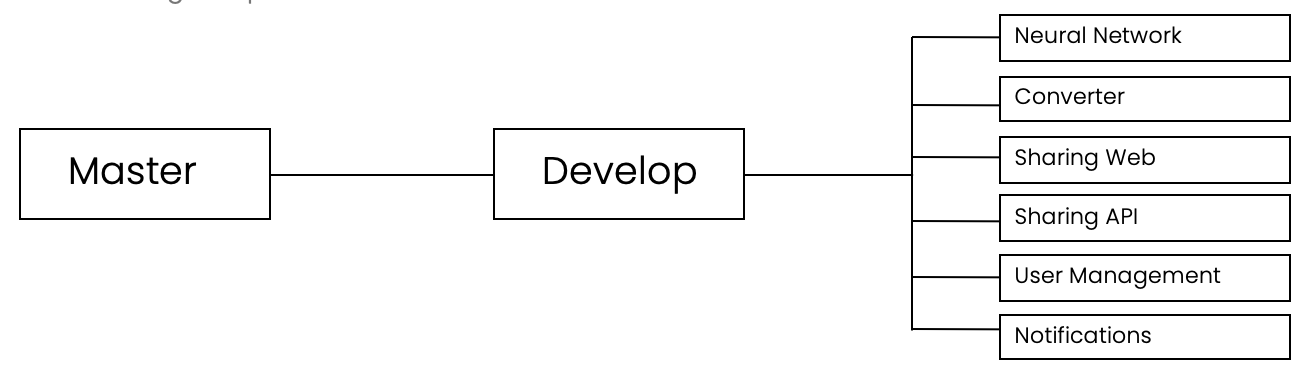
\includegraphics[width=10cm]{branches.png}
\end{figure}
\subsection{Folder structure}
\begin{itemize}
\item \textbf{app}
    \begin{itemize}
    \item Specific sub structure to be determined (read more below)
    \end{itemize}
\item \textbf{database}
    \begin{itemize}
    \item sharing
    \item usermanagement
    \end{itemize}
\item \textbf{documentation}
    \begin{itemize}
    \item androidfrontend
    \item converter
    \item integration
    \item neuralnetwork
    \item notification
    \item sharing
    \item usermanagement
    \item webfrontend
    \end{itemize}
\item \textbf{server}
    \begin{itemize}
    \item sharing
    \item usermanagement
    \item neuralnetwork
    \end{itemize}
\end{itemize}



\section{Project Management Tools}
\subsection{ClickUP (Project Management)}
Each team has been added to a unified ClickUP workspace where each team can see the progress of all other teams. Subtasks have been created by each team.

\begin{figure}[h]
    \centering
    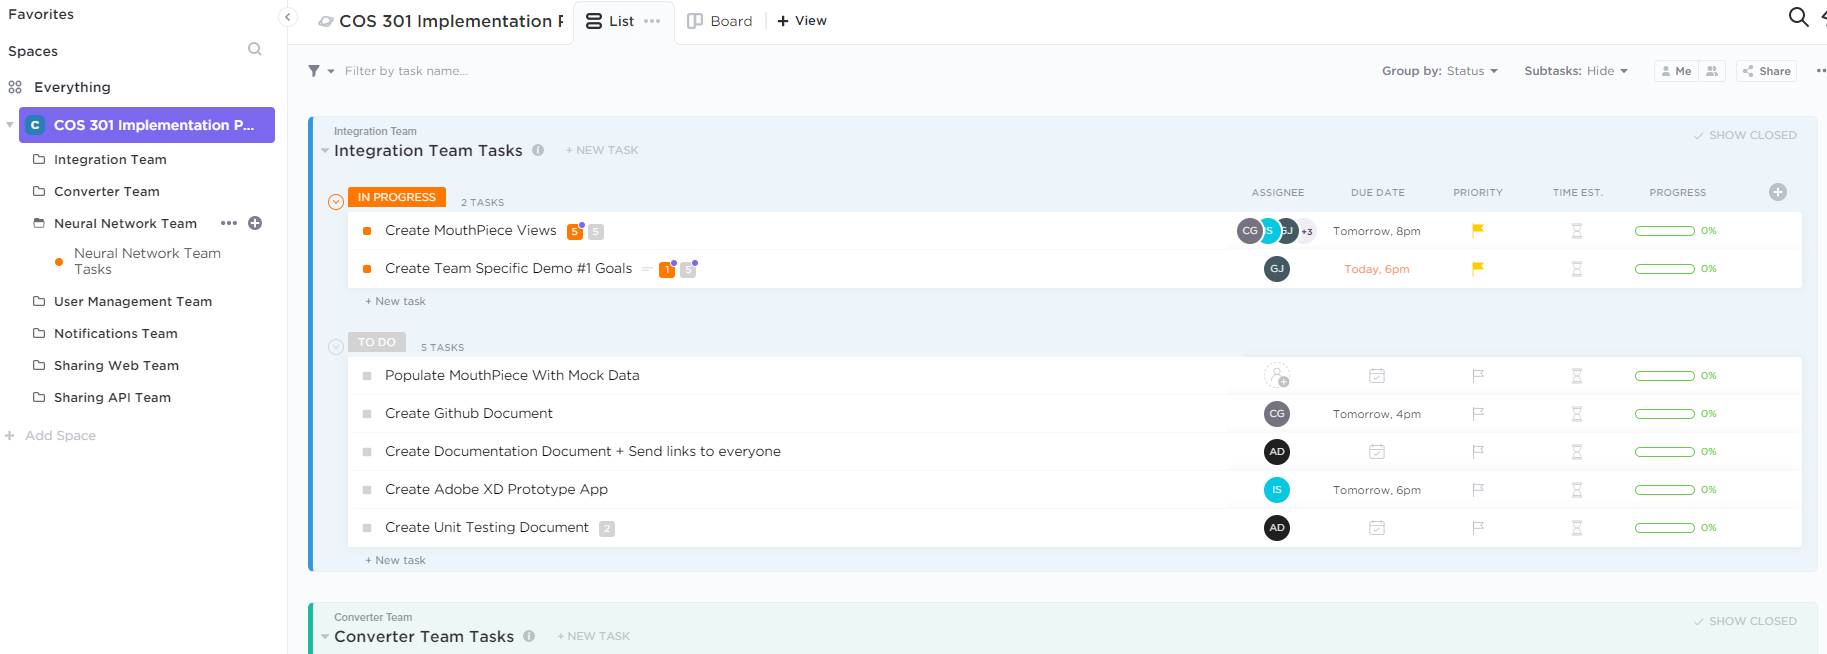
\includegraphics[width=\textwidth]{clickup.png}
\end{figure}

\subsection{Slack (Communication \& File Sharing)}
We have setup a Slack communication workspace where each team is added to a sub-channel as well as a global channel. 

\section{Technologies}
\begin{itemize}
    \item Flutter
    \item ClickUP (Team Management)
    \item Slack
    \item Github
\end{itemize}

\subsection{Mini Project DEMO \#1:}
\subsubsection{Mouthpiece App View Design}
We designed the different views of the Mouthpiece application and \\ implemented them in Flutter.

\begin{figure}[h!]
    \centering
    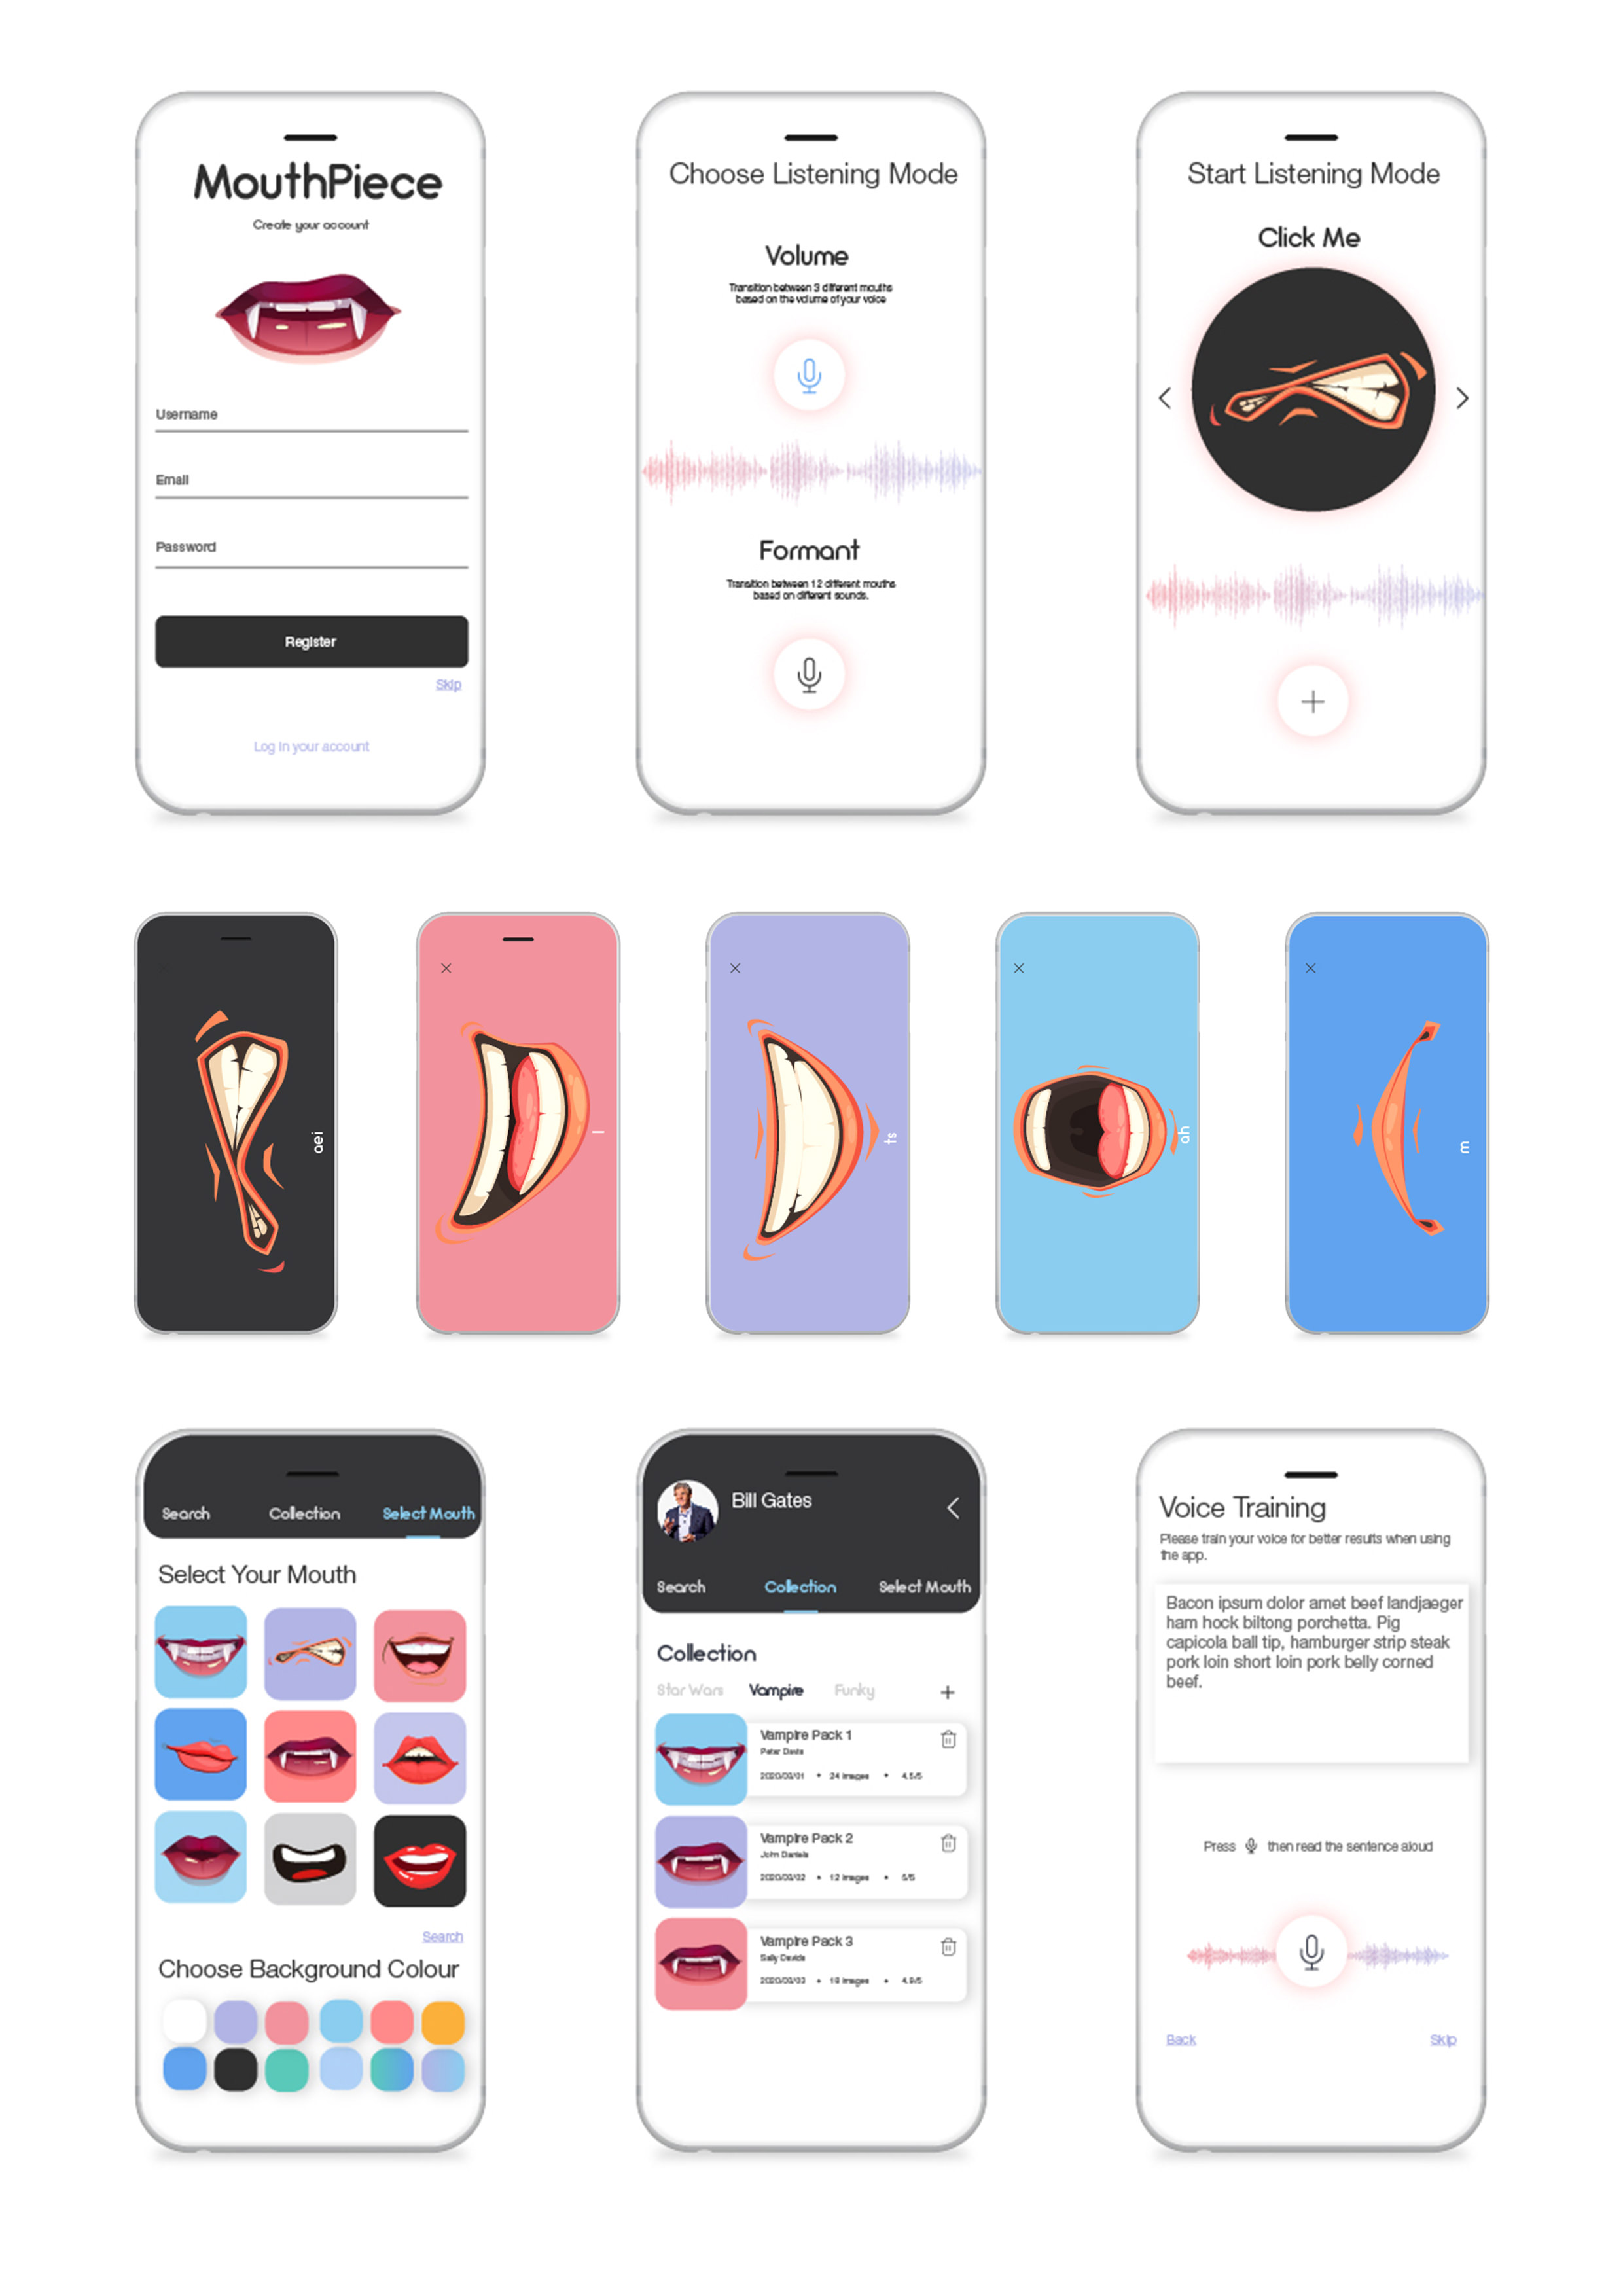
\includegraphics[width=11cm]{views.jpg}
    \caption{Mouthpiece App Views}
\end{figure}

\end{document}